\documentclass{article}
\usepackage{booktabs}
\usepackage{algorithm2e}
\usepackage{graphicx}
\title{LZW inspired De-Duplication algorithm for variable size blocks with sliding window}
\author{Justin}
\date{}
\begin{document}
   \maketitle
   \section{Introduction}
   The variable size defined in the title is a multiple of the smallest block size. So if the block size is 1 KB then the variable size blocks can be of 1, 2, 3 $\cdots$ KBs. Block size is set to 4 KB. So the block sizes will vary as a multiple of 4, ie. 4, 8, 12, 16, $\cdots$ 32 KB. An empty dictionary is used, as pre-calculating the hashes for all the blocks and adding to dictionary would be expensive on time and space. The dictionary is used only during de-duplication, and is not utilized while retrieving the original data from the de-duplicated data. A sliding block is also used in the algorithm to take into account blocks which might fall in between block boundaries. The window is advanced by an increment equal to $\Delta$d which is an integral multiple of the block size.
   \section{Algorithm - De-Duplication}
   
\begin{algorithm}[H]
 \KwIn{Data segment $\approx$ 200MB}
 \KwOut{Index, de-duplicated data segment}
 \Begin{
 Initialize: $p = false,\ size = 1,\ inc = \Delta d,\ blockPointer = 0,\ buffer = \phi$ \;
 \textbf{A:} Retrieve block at $blockPointer$, append retrieved block to buffer\;
 Calculate hash of the buffer\;
 \eIf{hash is in dictionary}{
 	set: $p=true$\;
 	$size+=1$ \;
 	$blockPointer += inc*x$\;
 	where $x$ is an integral multiple of block size $\equiv\ \Delta d = blockSize/x$\;
 	\eIf{End of segment}{
 		Goto \textbf{D}\;
 	}{
 		Goto \textbf{A}\;
 	}
 }{
 	Insert hash into dictionary\;
 	\eIf{$p=false$}{
 		$blockPointer += inc * x$\;
 		Goto \textbf{B}\;
 	}{
 		Generate index for previous non-unique block\;
 		$blockPointer += inc * x$\;
 		$p=false$\;
 		$size = 0$\;
 		$buffer=\phi$\;
 		\eIf{End of Segment}{
 			Goto \textbf{E}\;
 		}{
 			Goto \textbf{A}\;
 		}
 	}
 }
 \caption{De Duplication algorithm.}
 \label{deDupAlgo1}
 }
 \end{algorithm}
 \begin{algorithm}[H]
 %\Begin{
 \textbf{B:} Set $nextBlockPointer = blockPointer + (inc*x)$\;
 increment $blockPointer$ by $inc$\;
 set $prevBuffer = buffer$\;
 clear $buffer$\;
 \textbf{F:} Retrieve block at $blockPointer$\;
 Calculate hash\;
 \eIf{hash in dictionary}{
 	Output non-duplicate data between blocks, generate index\;
 	Goto \textbf{A}\;
 }{
 	Increment $blockPointer$ by $inc$\;
 	Clear buffer\;
 	\eIf{$blockPointer = nextBlockPointer$}{
 		decrement $blockPointer$ by $(inc*x)$\;
 		retrieve block at $blockPointer$ and append to $prevBuffer$\;
 		Calculate hash and add to dictionary\;
 		Goto \textbf{C}\;
 	}{
 		Goto \textbf{F}\;
 	}
 }
 \textbf{D:} Generate Index\;
 \textbf{E:} End\;
 
% }
 \caption{De Duplication algorithm. (cont.)}
 \label{deDupAlgo1}
\end{algorithm}

	
   
   \section{Re-duplication}
   \begin{enumerate}
   \item Start
   \item Read next/first entry of de-duplicated data.
   \item If data block: output as it is.
   \item Else if: index reference, then print blocks from the index till index+size.
   \item Last entry? if yes end, else goto step 2.
   \end{enumerate}
   \newpage
   
  \begin{figure}[h]
   \centering
    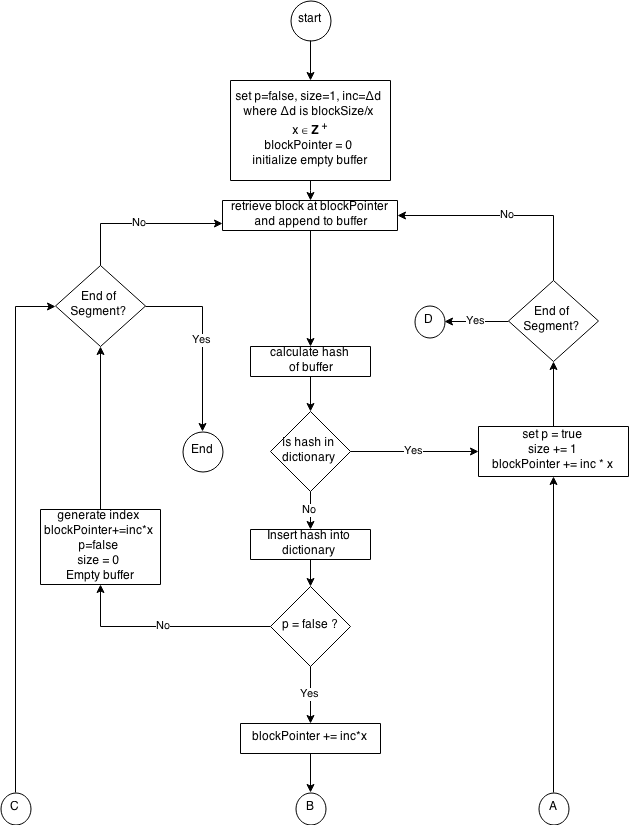
\includegraphics[scale=0.5]{deDup1.png}
    \caption{LZW inspired variable block de duplication}
   \end{figure}
   \begin{figure}
   \centering
    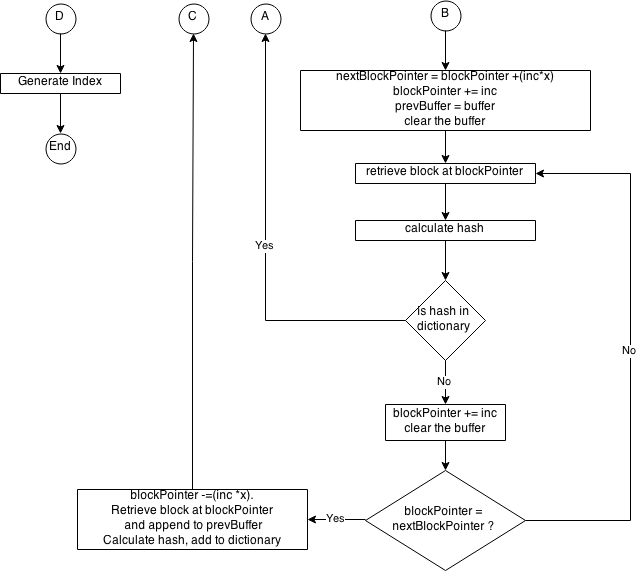
\includegraphics[scale=0.5]{deDup2.png}
    \caption{LZW inspired variable block de duplication (cont.)}
   \end{figure}
  \end{document}

